\section{extendedTerm - WIP}
% copied from  200806-ExtendedVersionComp

\textbf{Scenario} (sloppily copied from 200806-ExtendedVersionComp)
 \begin{center}
\begin{minipage}{.47\linewidth}
\centering
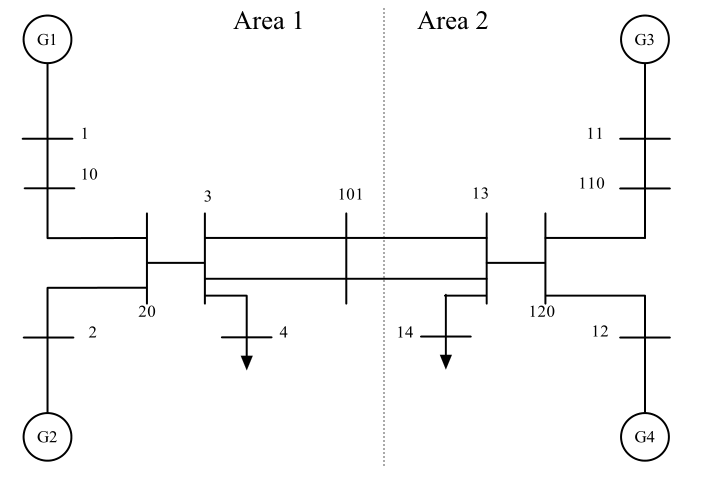
\includegraphics[width=\linewidth]{examples/extendedTerm/sysOneLineAreas}
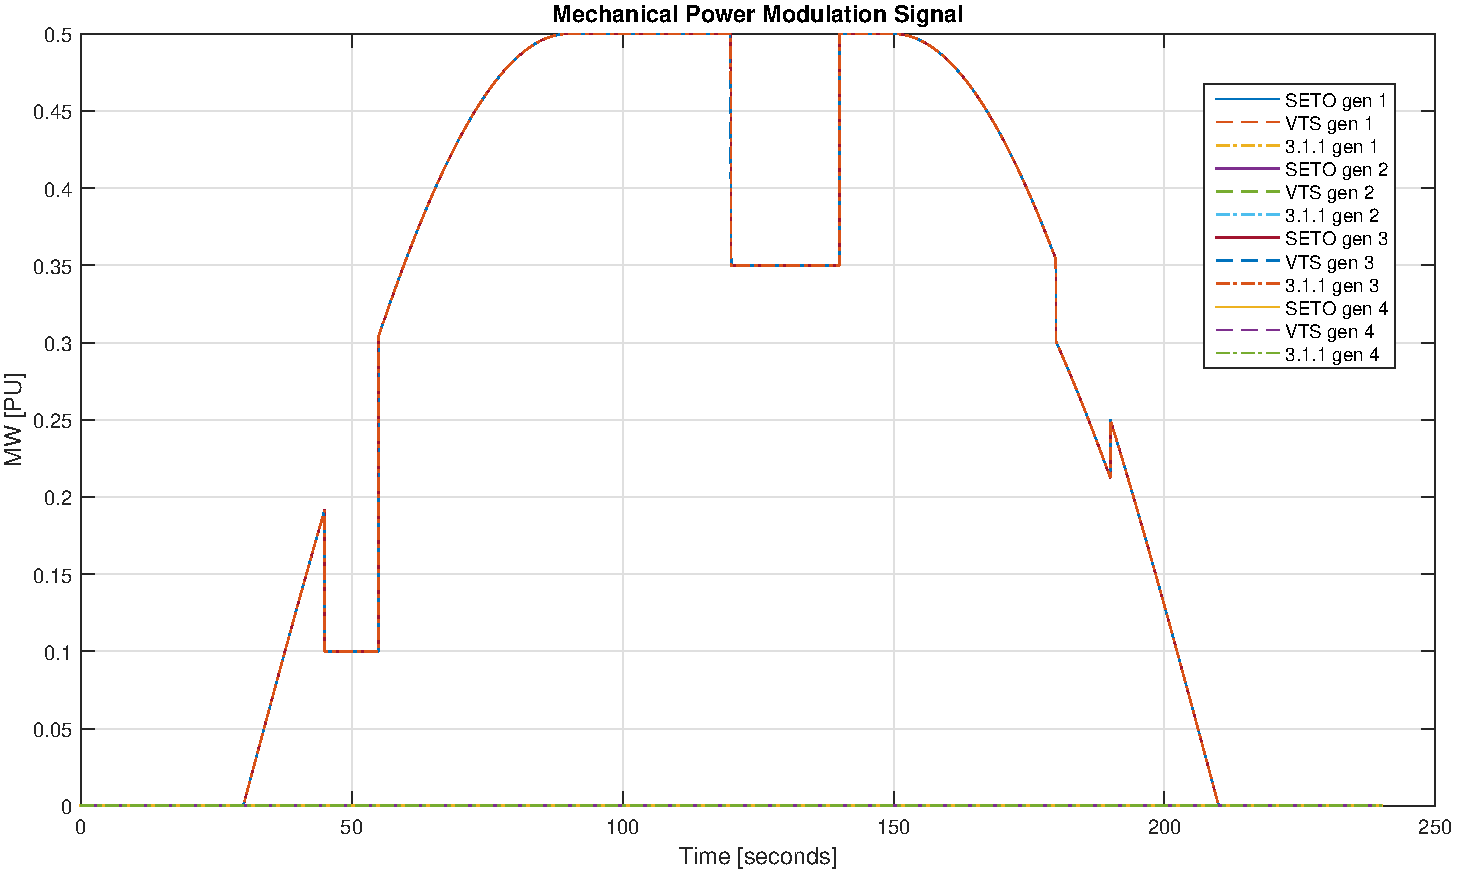
\includegraphics[width=.8\linewidth]{examples/extendedTerm/verPmSig}
\end{minipage} %
\begin{minipage}{.47\linewidth}
\begin{itemize}
\footnotesize
\itemsep 0em
\item Kundur  4 machine system packaged with PST
\item Constant Z load model
\item System has governors, exciters, and PSS.
\item Governor of generator being perturbed by pm\_sig removed
\item Perturbance was meant to mimic a solar ramp with various situations of cloud cover:\\
(larger plot of pm\_sig on Page 6)
\begin{Verbatim}[fontsize=\scriptsize]
% time [seconds]
% 0-30      - no action
% 30-90     - ramp up 0.5 PU (50 MW)
% 90-150    - hold peak
% 150-210   - ramp down 0.5 PU (50 MW)
% 210-240   - no action

% cloud cover events
% 45-55 - 20% max gen (generation of 0.1 PU)
% 120-140 - 30% cover (generation reduction to 70%)
% 180-190 - 15% cover (generation reduction to 85%)
\end{Verbatim}
\end{itemize}
\end{minipage}

\end{center}

\textbf{Summary} 
\begin{enumerate}
\itemsep 0 em
\item The PST 4 is 3.65 times faster than PST 3.1
\item Using variable time steps allows for a speed up of 14.84 over PST 3.1.
\item Results from all simulations are very similar.
\item Without creating an explicit time block at the beginning of an event, VTS events may not occur at the exact time they are programmed.
\item VTS reduces logged data size by $\approx$4 times.
\end{enumerate}


\begin{table}[!ht]
\resizebox{\linewidth}{!}{

	\begin{tabular}{@{} L{1.75cm} 
	R{2cm} R{2cm}  R{2cm} R{1.5cm} R{0.75cm} R{0.75cm} R{1.5cm} R{2cm} R{2cm}@{}} 	
		\toprule % @ signs to remove extra L R space
		\footnotesize % this will affect the table font (makse it 10pt)
		\raggedright % for non justified table text

	&	\multicolumn{3}{c}{Step Size [seconds]}					&		&	\multicolumn{2}{c}{Solutions Per Step}			&		&		&		\\	
\shortstack{PST\\Version}	&	Max.	&	Min.	&	Ave.	&	Total Steps	&	Ave.	&	Max.	&	Total Slns.	&	Sim. Time	&	Speed Up	\\ \midrule	
3.1	&	4.00E-03	&	4.00E-03	&	4.00E-03	&	59,975	&	2	&	2	&	119,950	&	916.24	&	1.00	\\	
4.0	&	4.00E-03	&	4.00E-03	&	4.00E-03	&	59,975	&	2	&	2	&	119,950	&	250.82	&	3.65	\\	
VTS	&	2.32E+01	&	2.68E-04	&	2.58E-02	&	9,315	&	2	&	97	&	17,006	&	61.73	&	14.84	\\	
																				\bottomrule
	\end{tabular}
	}%end resize box
	



\end{table}


\pagebreak
% fixed: 8749 steps i.e., 17498 network solutions 

%>> compareVTSandFTS
%VTS time: 15.8579
%fixed time: 57.4479
 

\textbf{Plotted Results - Step Size / Number of Solutions Comparison} \ \\
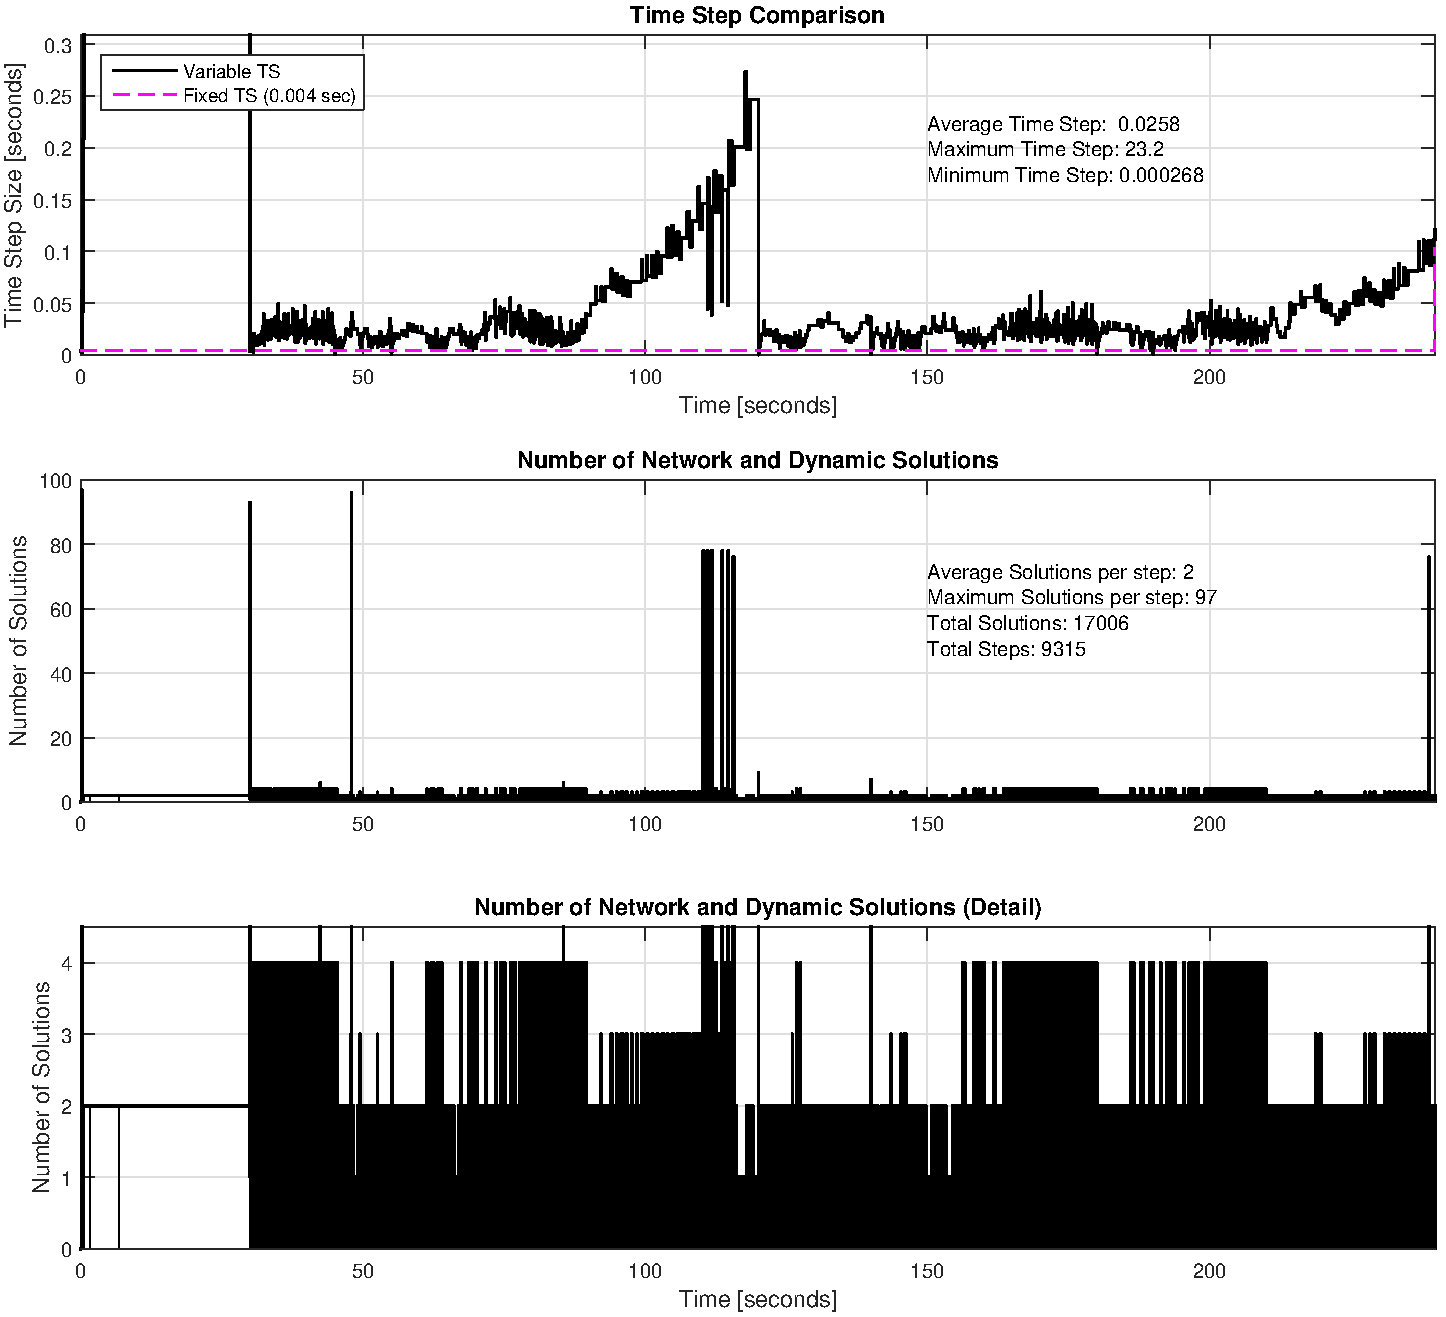
\includegraphics[width=\linewidth]{examples/extendedTerm/verSteps}

NOTE: Initial time steps before t=30 are much larger than the other time steps (multiple seconds) and are plotted off the axis.

\pagebreak
\textbf{Plotted Results - Various Comparisons} \ \\
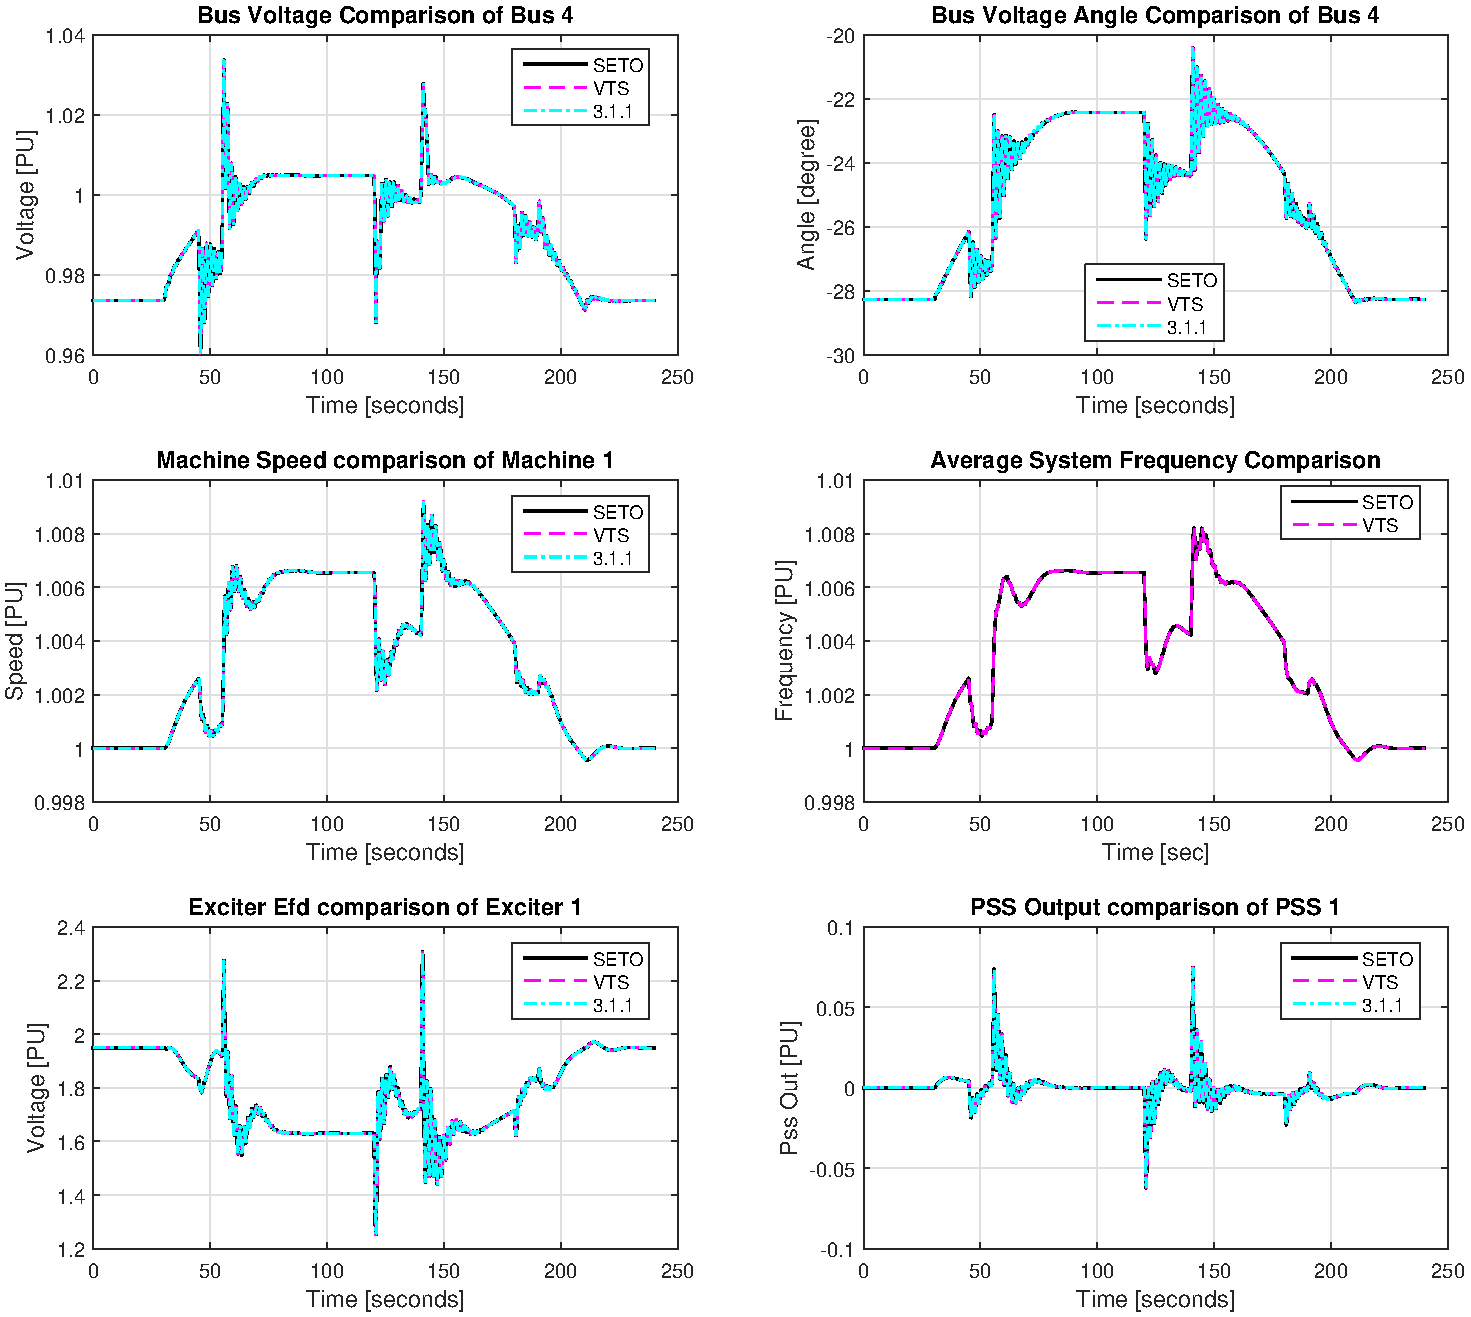
\includegraphics[width=\linewidth]{examples/extendedTerm/verComp}

NOTE: 3.1 does not calculate average system frequency.

\pagebreak
\textbf{Plotted Results - Various Comparisons - Detail 1} \ \\
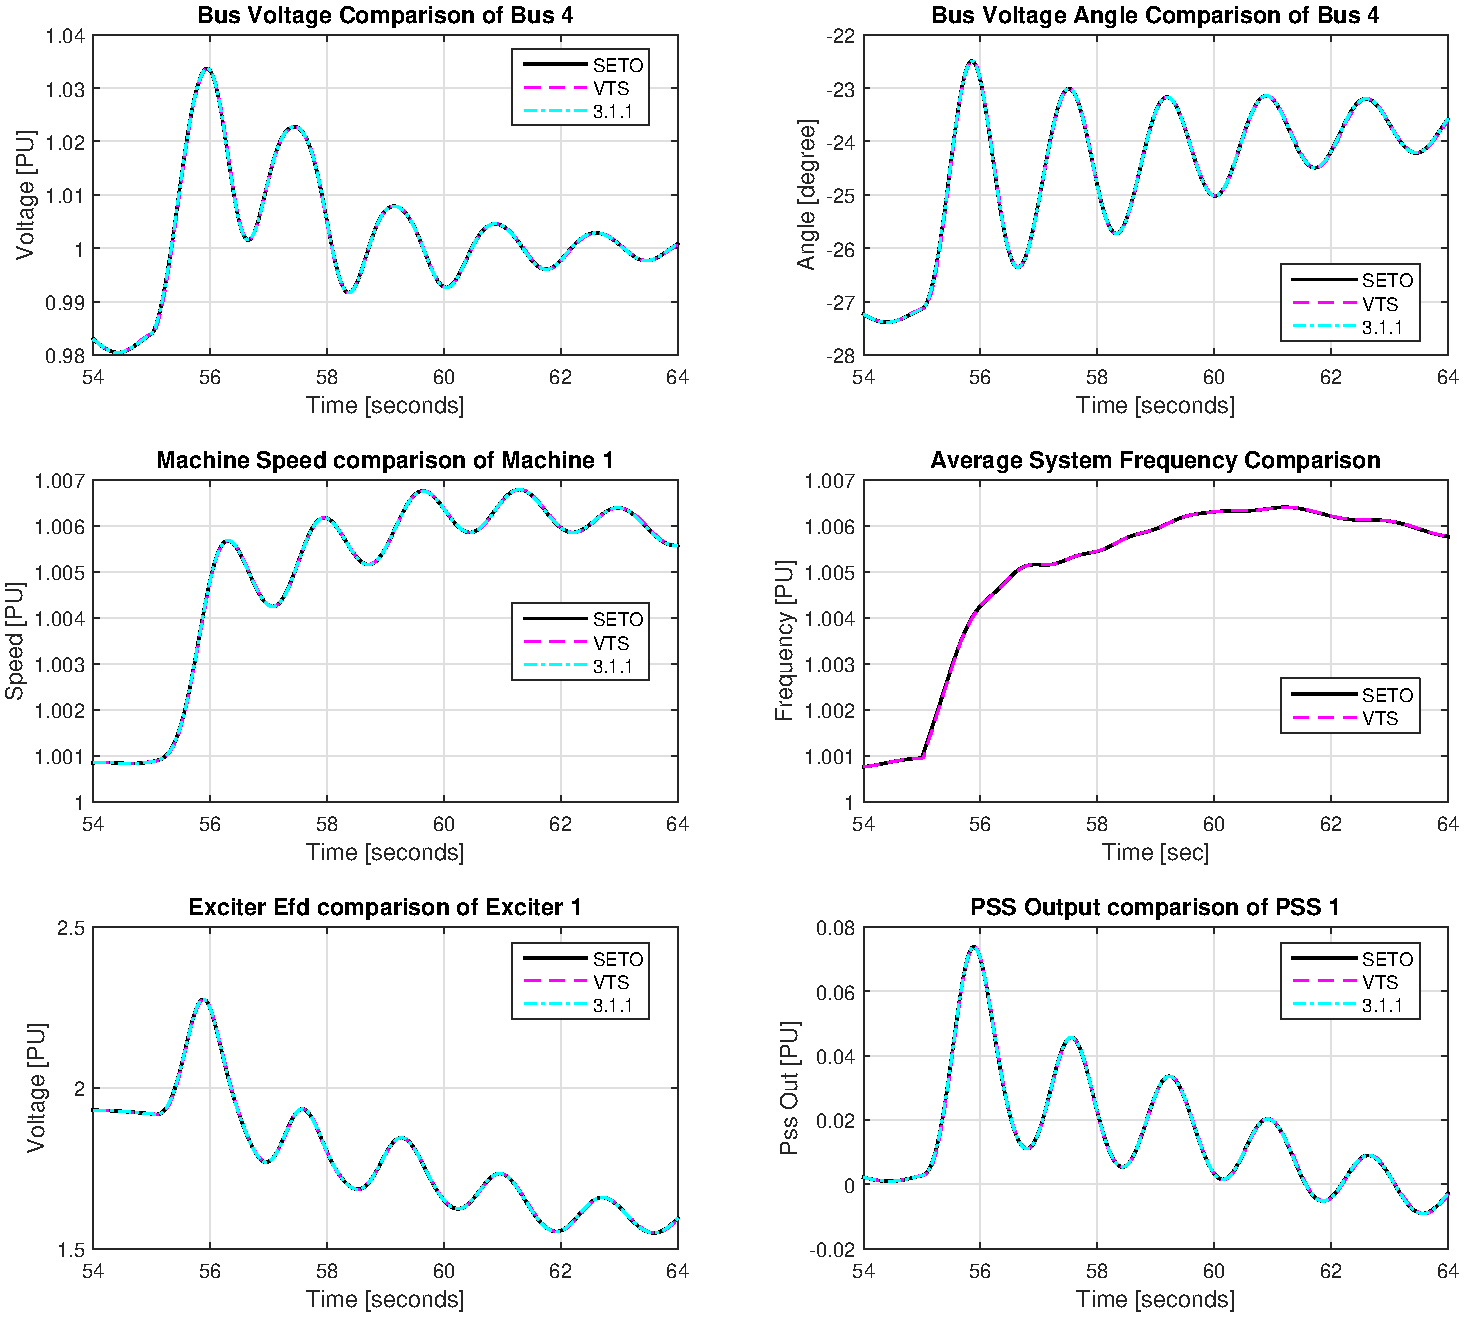
\includegraphics[width=\linewidth]{examples/extendedTerm/verCompDetail1}

NOTE: 3.1 does not calculate average system frequency.

\pagebreak
\textbf{Plotted Results - Various Comparisons - Detail 2} \ \\
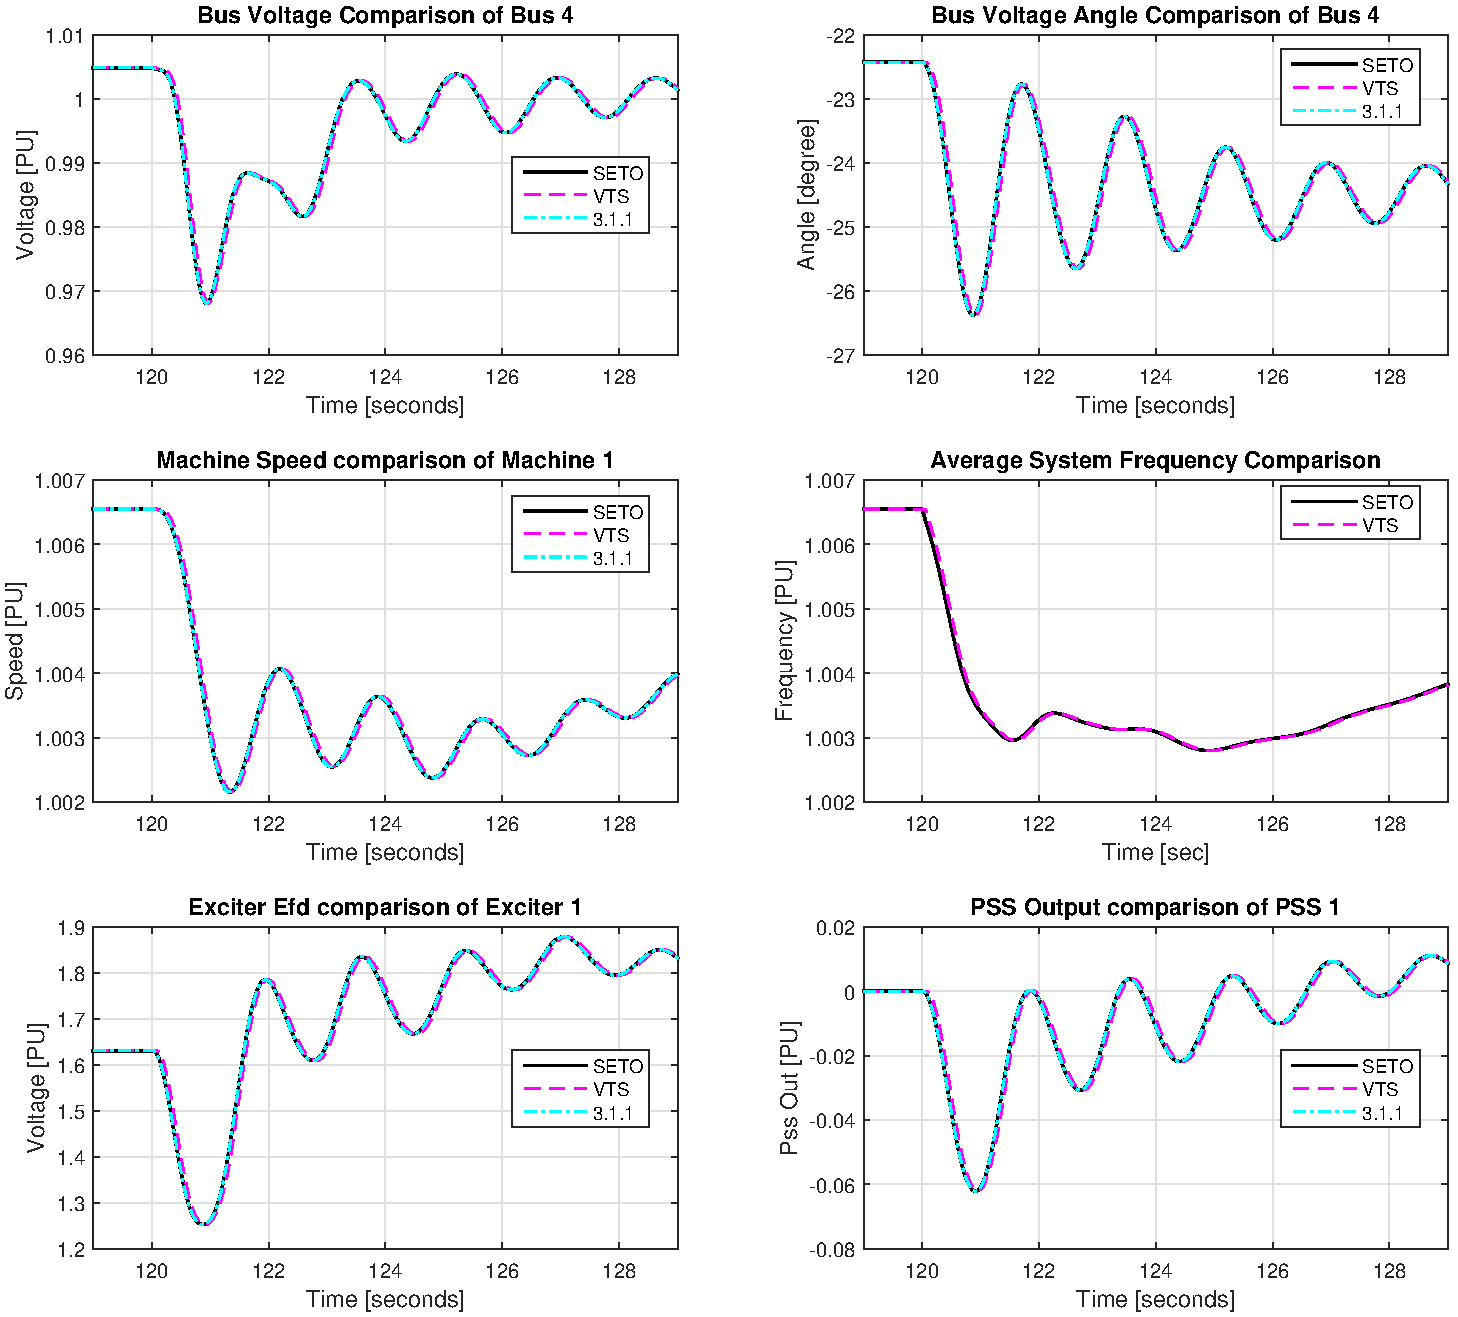
\includegraphics[width=\linewidth]{examples/extendedTerm/verCompDetail2}

NOTE: 3.1 does not calculate average system frequency.

VTS events may not occur at exact specified time due to the nature of variable time steps.

Breaks in the \verb|sw_con| can be created to account for this, however, the variance in time is often relatively small.


\pagebreak
\textbf{Plotted Results - Modulation Signal} \ \\
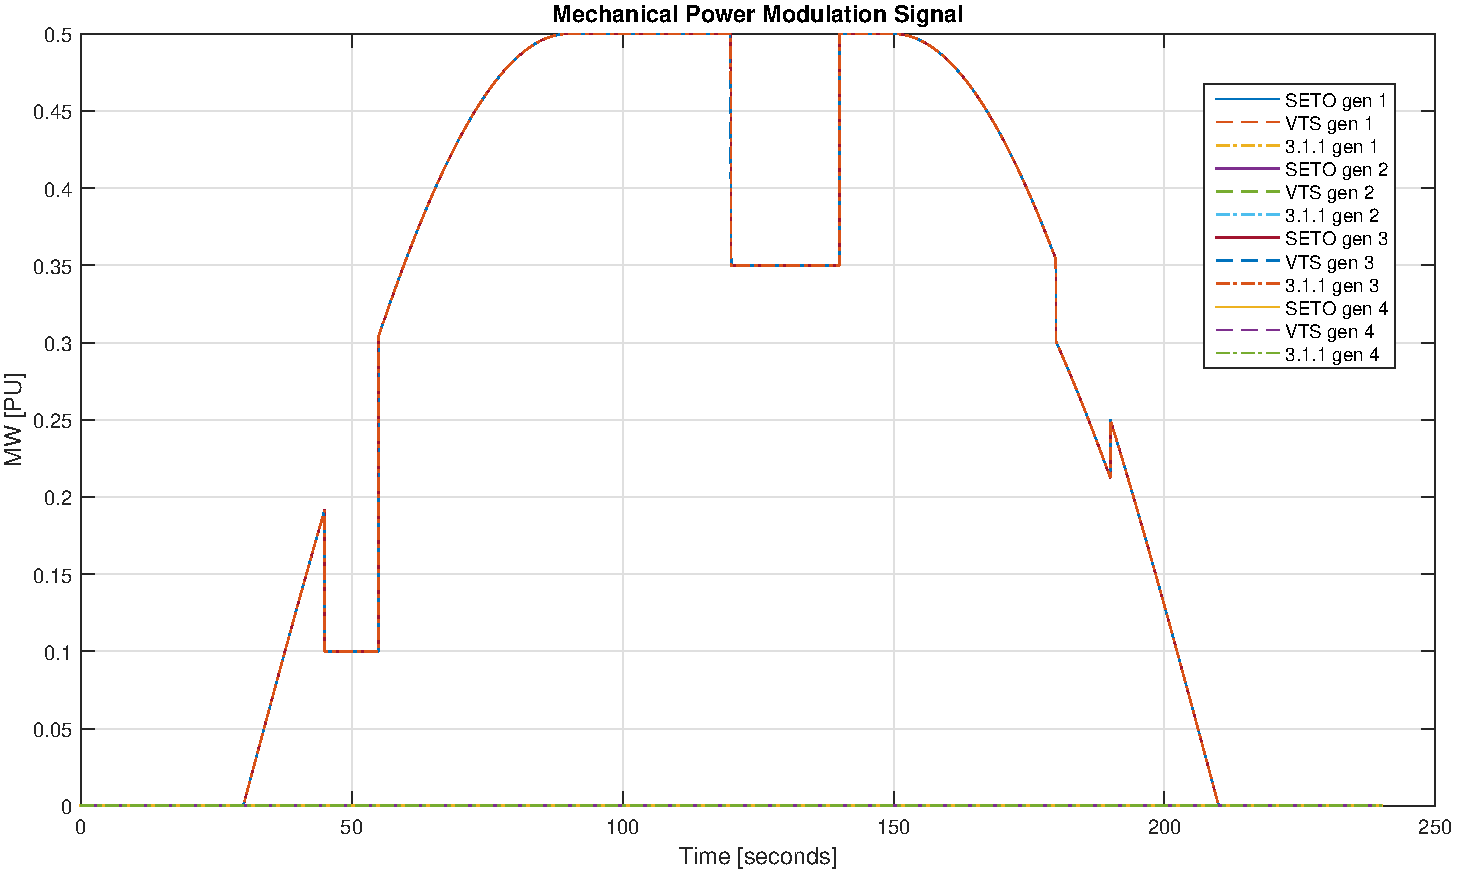
\includegraphics[width=\linewidth]{examples/extendedTerm/verPmSig}
\textbf{Plotted Results - Mechanical Power} \ \\
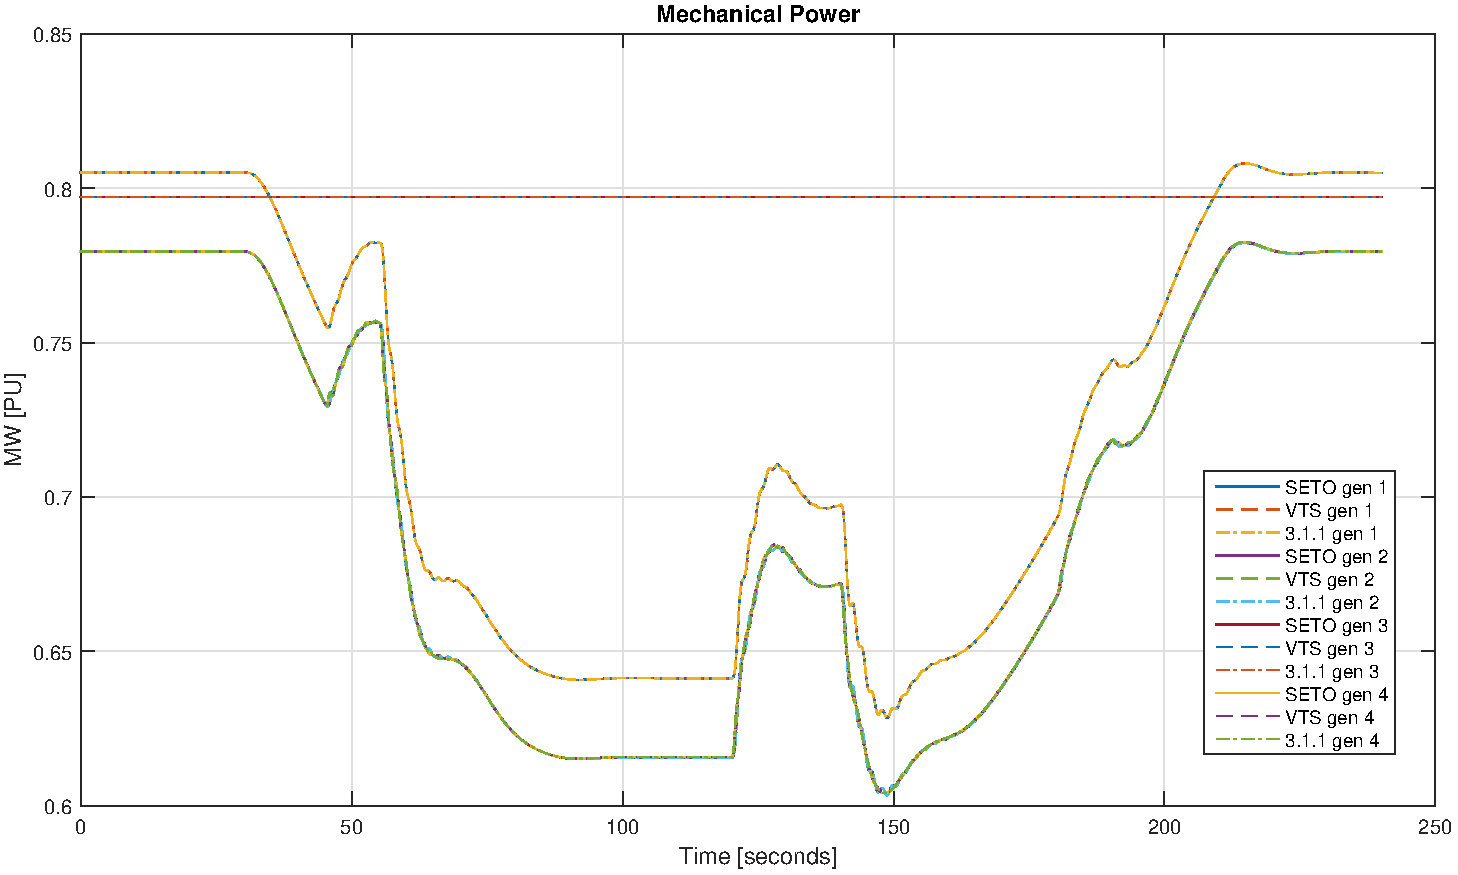
\includegraphics[width=\linewidth]{examples/extendedTerm/verPmech}
Note that the modulated mechanical power signal is not added to the recorded mechanical power.
\textbf{Plotted Results - Electric Power} \ \\
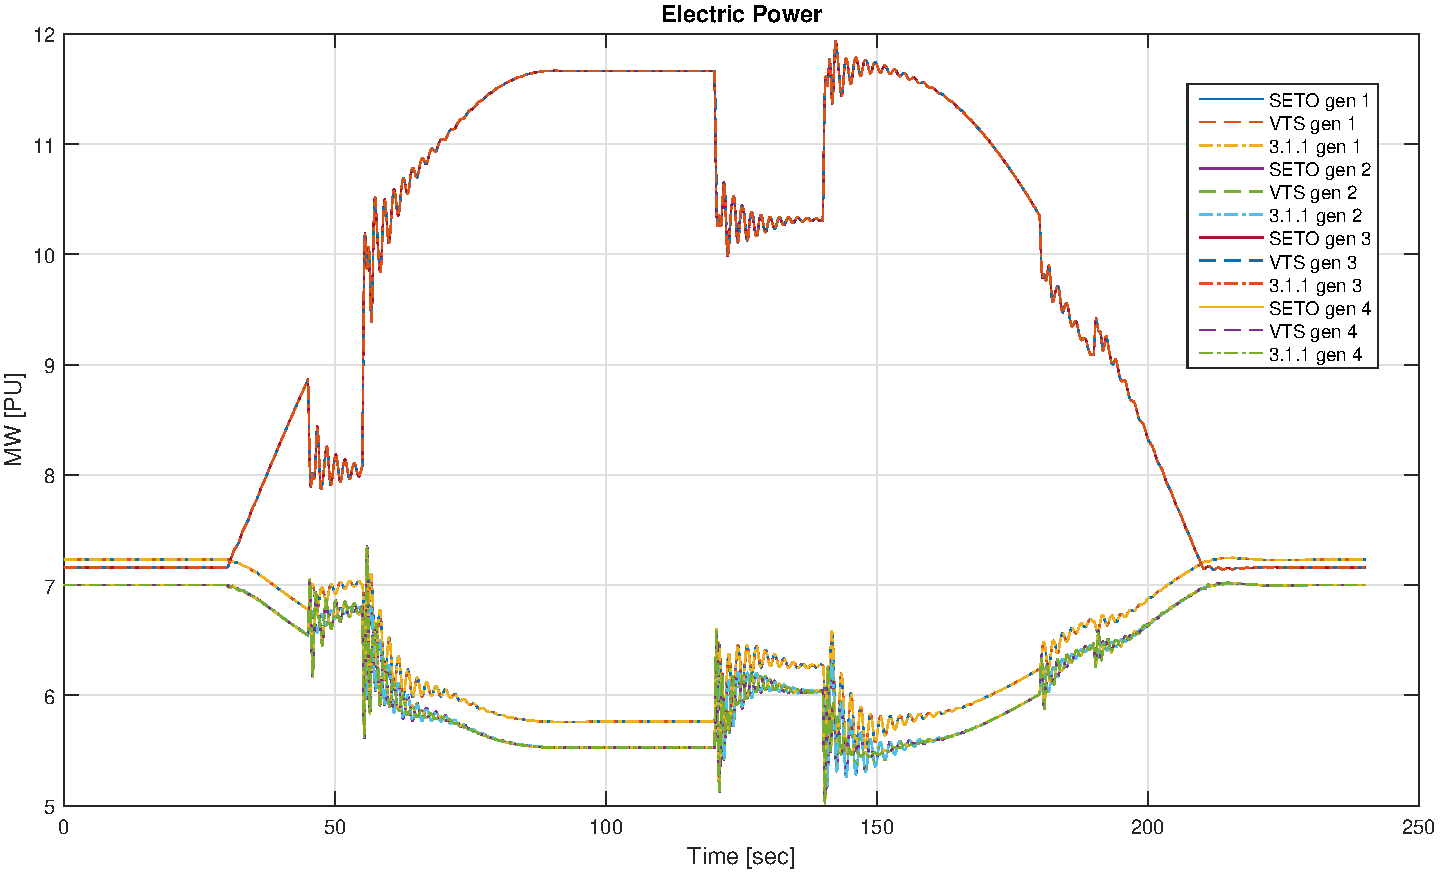
\includegraphics[width=\linewidth]{examples/extendedTerm/verPelect}

\textbf{Plotted Results - Electric Power - Detail} \ \\
Detail of generators 1, 2, and 5 from t= 140 to 150:\\
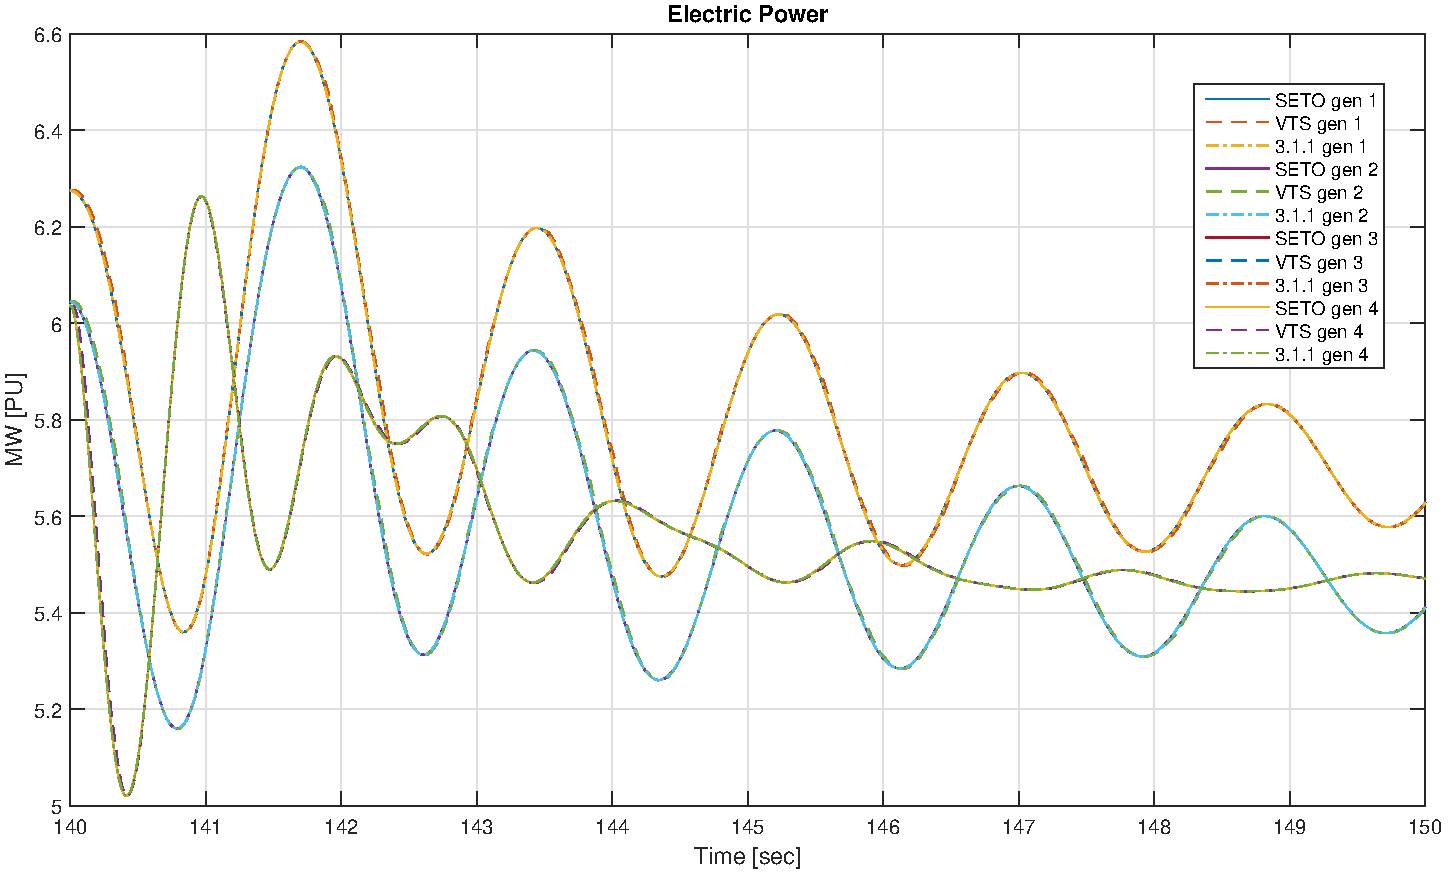
\includegraphics[width=\linewidth]{examples/extendedTerm/verPelectDetail}